\input{preamble}

\usepackage{booktabs}

\begin{document}

\setlist{noitemsep}  % Reduce space between list items (itemize, enumerate, etc.)
\onehalfspacing      % Use 1.5 spacing
% Use endnotes instead of footnotes - redefine \footnote command
%\renewcommand{\footnote}{\endnote}  % Endnotes instead of footnotes

\author{Rasmus M. Jensen \& Morten B. Krogh\thanks{\rm Jensen \& Krogh are both Master Students at Aarhus School of Business and Social Sciences, Aarhus University. We thank our suporvisor Stig Vinther Møller for making this project possible with passionate and inspirational guidance.}}

\title{\Large \bf Business Cycles and predictability of Returns under habit Formation}

\date{}              % No date for final submission

% Create title page with no page number

\maketitle
\thispagestyle{empty}

\bigskip

\centerline{\bf ABSTRACT}

\begin{doublespace}  % Double-space the abstract and don't indent it
  \noindent We recalibrate the model of \citet{Campbell1999} on up-to-date US-data and simulate 100.000 months of returns in order to examine whether the model is able to generate data that is predictable during recessions. In addition we provide results on the overall out-of-sample predictability of stock returns generated from an external habit model.
\end{doublespace}

\medskip

\noindent \textit{Keywords: Consumption-based asset pricing, Habit formation.} \\

\noindent JEL classification: G11, G12, G32

           
  

\clearpage

\section{Introduction} \label{sec:Introduction}

\begin{comment}
idé gør som Cochrane og Campbell 1999:
\begin{enumerate}
    \item Kalibrer modellen (Mikrofundament)
    \item Simulér variable og PD
    \item Lav Recesssionsdummy fra surplus consumption / consumption
    \item Cross-sectional regressions med dummies
    \item Kan man forecaste OoS returns under recession og ikke expansion <- theoretical
\end{enumerate}

\hline

\begin{enumerate}
    \item evidence for predictability in recessions is already established, however due to the fact that the state of the economy only is recession approximately 10\% of the time, we find it interesting to investigate the power of the model in expansions as well. 
    \item This investigation will be conducted relaying heavily upon \cite{Campbell1999} and using a regime switchin regression framework. 
    \item The recession dummy will be construted from the surplus consumption ration simple as follows
    \begin{align}
        rec_t & = \begin{cases} 1 & \text{, if } s_t < \Bar{s} \\
                              0 & \text{, if } s_t > \Bar{s} \end{cases}
    \end{align}
    
    and the regression equation below
    
    \begin{align}
        r_{t+h} & = \alpha + \beta_1 \times r_t + \underbrace{\beta_2 \times pd_t  \times I_{rec_t}}_{\text{recession indicator}} + \underbrace{\beta_3 \times pd_t \left(1 - I_{rec_t} \right)}_{\text{Expansion Indicator}} + \varepsilon_{t+h} 
    \end{align}
    
    skriv noget om hvad andre har fundet ud af, nævn stigs 2013 artikel ifm. bond return predictability og nævn andre campbel osv der finder unpredictability i returns.

\end{enumerate}




This paper investigates the Habit Formation model proposed by \cite{Campbell1999} ability to predict in expansions as well as the out-of-sample performance of the model. 
The history of Asset Pricing models have provided evidence of predictability in periods of economic downturn \colorbox{yellow}{\textbf{INDSÆT KILDER}}, however, there have been little evidence showing predictability in expansions. The ability to predict in expansions are a highly desired capability, due to the fact the economy historically is in the state of expansion more often than recession. In the \cite{Campbell1999} framework, recession is defined as period where surplus consumption is below steady-state, hence the models recession is not exactly equal to the definition of three quarters of negative GDP growth as we are used to...


\hline

We examine the \cite{Campbell1999} model of Habit formation in asset pricing. Investigating the models performance both in recessions, which multiple sources have provided evidence of predictability of returns, and in expansions where it has been the case to be more difficult to predict returns. 

We calibrate the model based on newer data than \cite{Campbell1999}, then we perform a simple regression with an indicator variable of recession and $(1-I_{rec}$ for expansions, this is done for the ability to distinguish between model performance in recessions as well as in expansions. 

A recession in the model is defined as when surplus consumption is below some given value, that is 

    \begin{align}
        I_{rec} & = \begin{cases} 1 & \text{, if } s_t < s_{rec} \\
                                  0 & \text{, if } s_t > s_{rec} 
                    \end{cases}
    \end{align}

in order to match the empirical amount of times the economy have been in recession according to \cite{USREC} in the period $1950 - 2018$ $\approx 13 \%$, the threshold $s_{rec}$ needs to take a value somewhere below $s_{bar}$, otherwise if $s_{bar}$ is used as threshold the economy of the model will be in recession approximately $37\%$ of the time, this three times more than the economy actually have been in the last 68 years, thus the need for lowering the threshold. The threshold value of the surplus consumption ratio is found by integrating over the stationary distribution of the surplus consumption ratio.




We show that the model of \citet{Campbell1999} is capable of generating returns consistent with the empirical findings of \citet{Henkel2011}. That is returns which inherits the properties that they are predicable in recession but unpredictable in expansions.\\

\citet{Henkel2011} found that the predictability of returns using popular measures such as the dividend yield diminishes in expansions while remaining of significance during recessionary periods. \\

We simulate an economy according to \cite{Campbell1999}, and re-calibrate the parameters of the model to an extended period spanning \textit{1950-2018} compared to \citep{Campbell1999}'s \textit{1950-1994}. In an attempt to incorporate relevant information of the Great Financial Crisis of 2008 in our calibration.




Predictability of asset prices in expansions is a desirable capability since the economy is in a state of expansion more often than recession. In the period $1950-2018$\footnote{According to \cite{USREC}} the economy has been in recession $13.41\%$ of the time, hence being able to predict asset prices in expansions would yield a higher profit for investors.
\end{comment}

%\begin{comment}
A corner area of the consumption based asset pricing is to incorporate habits in an agents preferences, \textit{Habit Formation}. The idea, initiated by \citet{Constantinides_1990}, assumes that marginal utility of consumption rely on consumption relative to stochastic habit process which is related to past consumption, thus utility is a function of both consumption and habits $u \left(C_t, X_t \right)$. This captures a fundamental psychological feature of human behavior, namely when income rises consumption only slowly adapts, thus being exposed to a stimulus again and again reduces the response. 

\citet{Campbell1999} considers a model with external habit, that is habit depends on aggregate consumption, and thus is unaffected by a single agents choices, this type of habit is also refereed to as \textit{>>catching up with the Joneses<<}. They specify the consumption utility function as a power function of differences $C_t - X_t$ and are able to match empirical features of the economy such as the excess return on stocks, the sharpratio and riskfree rate to mention a few. 

In this paper we follow \citet{Campbell1999} approach and are able to reproduce their results, then we re-calibrate the parameters of the model by extending the period spanning  $1950 \ -  \ 2018$, this includes the both the \textit{>>dot com bubble<<} in 2000 and the \textit{>>Great Financial Crisis<<} in 2007-2009, incorporating this period is an attempt to capture more recent and relevant information in the calibration. We define an indicator for recession to match the amount of times the economy has been in recession in the data period \textit{13.4\%}, and estimate both the ordinary asset pricing regression where we divide effects of predictability into recession- and expansion periods, besides this we also estimate a regime switching regression where the left hand side is conditioned upon the indicator. 
The results show that the model of \citet{Campbell1999} is capable of generating returns consistent with the empirical findings of \citet{Henkel2011}. That is returns which inherits the properties that they are predicable in recession but unpredictable in expansions.

%\end{comment}
% \section{Data} \label{sec:Data}

For calibration of the model parameters we use the CRSP U.S. Stock data for monthly, quarterly and annual observations of returns with and without dividends. 

\section{Methodology} \label{sec:Methodology}
\section{Analysis} \label{sec:Analysis}

\subsubsection{Calibrated Model}

\begin{table}[H]
\center
\begin{threeparttable}[b]
\caption{Parameters of the model}
\label{tab:ModelCalib}
\begin{tabular}{@{}ll@{\hspace{1.5cm}}ll@{}}
\toprule
 & Parameter                              & Notation         & Value    \\ \midrule 
\multicolumn{4}{l}{\textit{Calibrated}}                                 \\
 & Mean consumption growth                & $g$              & $0.0134$ \\
 & Standard deviation of $\Delta c_t$     & $\sigma$         & $0.0152$ \\
 & Standard deviation of $\Delta d_t$     & $\sigma_w$       & $0.1256$ \\
 & Log risk-free rate                     & $r^f$            & $0.0109$ \\
 & Persistence parameter                  & $\phi$           & $0.9008$ \\
 \multicolumn{4}{l}{\textit{Assumed}}                                   \\
 & Coefficient of Risk Aversion           & $\gamma$         & $2.0000$ \\
 & Correlation dividends/consumption      & $\rho$           & $0.2000$ \\
\multicolumn{4}{l}{\textit{Implied}}                                    \\
 & Subjective discount factor             & $\delta$         & $0.9156$ \\
 & Steady-state surplus consumption ratio & $\Bar{S}$        & $0.0666$ \\
 & Maximum surplus consumption ratio      & $S_{\text{max}}$ & $0.1096$ \\ \bottomrule
\end{tabular}
\begin{tablenotes}
\footnotesize{\item [1] All relevant parameters are annualized
              \item [2] Calibrated parameters are estimated from data, assumed are chosen arbitrarily on the grounds of existing literature, while implied parameters are calculated from the calibrated/assumed parameters.}
\end{tablenotes}
\end{threeparttable}
\end{table}

%\begin{table}[H]
\centering
\begin{threeparttable}[b]
\caption{Parameters of the model}
\label{tab:ModelCalib}
\begin{tabular}{@{}ll@{\hspace{1.5cm}}ll@{}}
\toprule
 & Parameter                              & Notation         & Value    \\ \midrule
\multicolumn{4}{l}{\textit{Calibrated}}                                 \\
 & Mean consumption growth                & $g$            & $0.0134$ \\
 & Standard deviation of $\Delta c_t$     & $\sigma$         & $0.0152$ \\
 & Standard deviation of $\Delta d_t$     & $\sigma_w$       & $0.1256$ \\
 & Log risk-free rate                     & $r^f$            & $0.0109$ \\
 & Persistence parameter                  & $\phi$           & $0.9008$ \\
 \multicolumn{4}{l}{\textit{Assumed}}                                   \\
 & Coefficient of Risk Aversion           & $\gamma$         & $2$ \\
 & Correlation dividends/consumption      & $\rho$           & $0.2$ \\
\multicolumn{4}{l}{\textit{Implied}}                                    \\
 & Subjective discount factor             & $\delta$         & $0.9156$ \\
& Steady-state surplus consumption ratio & $\Bar{S}$        & $0.0666$ \\
 & Maximum surplus consumption ratio      & $S_{\text{max}}$ & $0.1096$ \\ \bottomrule
\end{tabular}
\begin{tablenotes}
\footnotesize{\item [1] All relevant parameters are annualized
              \item [2] Calibrated parameters are estimated from data, assumed are chosen arbitrarily on the grounds of existing literature, while implied parameters are calculated from the calibrated/assumed parameters.}
              
\end{tablenotes}
\end{threeparttable}
\end{table}
\begin{table}[H]
\centering
\begin{threeparttable}[b]
\caption{Parameters of the model}
\label{tab:ModelCalib}
\begin{tabular}{@{}ll@{\hspace{1.5cm}}ll@{}}
\toprule
 & Parameter                              & Notation         & Value    \\ \midrule
\multicolumn{4}{l}{\textit{Calibrated}}                                 \\
 & Mean consumption growth                & $g$            & $0.0134$ \\
 & Standard deviation of $\Delta c_t$     & $\sigma$         & $0.0152$ \\
 & Standard deviation of $\Delta d_t$     & $\sigma_w$       & $0.1256$ \\
 & Log risk-free rate                     & $r^f$            & $0.0109$ \\
 & Persistence parameter                  & $\phi$           & $0.9008$ \\
 \multicolumn{4}{l}{\textit{Assumed}}                                   \\
 & Coefficient of Risk Aversion           & $\gamma$         & $2$ \\
 & Correlation dividends/consumption      & $\rho$           & $0.2$ \\
\multicolumn{4}{l}{\textit{Implied}}                                    \\
 & Subjective discount factor             & $\delta$         & $0.9156$ \\
& Steady-state surplus consumption ratio & $\Bar{S}$        & $0.0666$ \\
 & Maximum surplus consumption ratio      & $S_{\text{max}}$ & $0.1096$ \\ \bottomrule
\end{tabular}
\begin{tablenotes}
\footnotesize{\item [1] All relevant parameters are annualized
              \item [2] Calibrated parameters are estimated from data, assumed are chosen arbitrarily on the grounds of existing literature, while implied parameters are calculated from the calibrated/assumed parameters.}
\end{tablenotes}
\end{threeparttable}
\end{table}



Compared to the calibration of \citet{Campbell1999}, our calibration suggests a higher persistence parameter, higher volatility of dividend growth and lower consumption growth, the implied surplus consumption parameters suggests a slightly higher overall surplus consumption. The differences likely stems from the extra 20 years of calibration data. \\
\subsection{Simulation}
From the calibrated model we simulate a chain of 100.000 monthly draws from the economy yielding 8.332 years of simulated time-series. Allowing us to infer about the predictability of excess stock returns, during times of simulated crisis. \\
\newline
Based upon NCER-recession data, we find that the US economy was in recession approximately 13.4\% of the period spanning January 1950 until December 2018.  In the model a recession implies that present consumption in low relative to previous periods consumption, that is the value of $s_t$ is lower than the steady state value of surplus consumption $\Bar{s}$ - integrating over the density of $s_t$ yields that the simulated economy is in recession during 37\% of all observations, which indicates that $\Bar{s}$ might be misspecified. To correct $\Bar{s}$ we match the empirical business cycle behavior by numerical optimization of the $s_t$ density, such that the empirical and simulated economy is in recession roughly the same amount. The $\Bar{s}$-value matching the empirical business cycle, throughout denoted $\Bar{s}_{rec}$ \textit{or} ($\Bar{S}_{rec}$), is found to be $-3.18$ ($0.0415$).

\begin{figure}[H]
    \centering
    \caption{Distribution of simulated $s_t$ chain}
    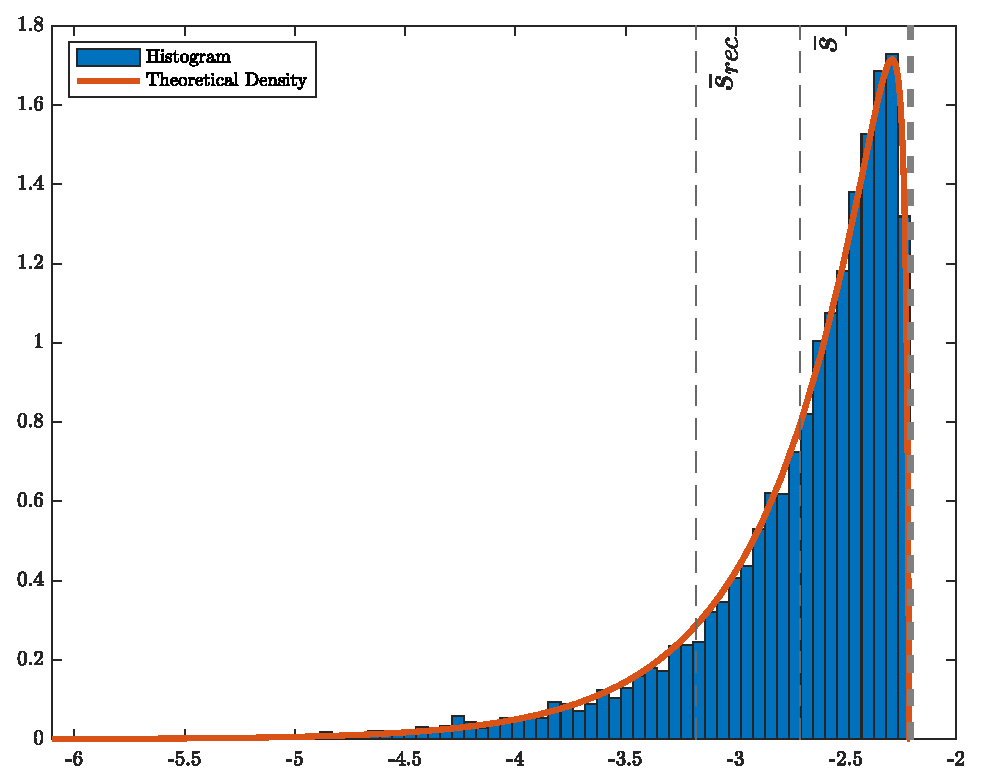
\includegraphics[width=\textwidth]{Figures/DistributionS_t.eps}
    \label{fig:DistriSt}
\end{figure}

\begin{table}[H]
\centering
\caption{Data Properties}
\label{tab:Data_props}
\begin{tabular}{@{}l@{\hspace{1.5cm}}l@{\hspace{1.5cm}}l@{}}
\toprule
 & \textit{Simulated} & \textit{Historic} \\ \midrule
$\mathbb{E}\left[r_t- r^f_t\right]$& $0.0373$           & $0.0927$          \\
$\sigma\left(r_t - r^f_t  \right)$ & $0.0962$           & $0.1670$          \\
$\mathbb{E}\left[r_t- r^f_t\right] / \sigma\left(r_t - r^f_t,\right)$ & $0.3877$ & $0.5548$  \\ \bottomrule
\end{tabular}
\end{table}

%\begin{table}[H]
\centering
\caption{Data Properties}
\label{tab:Data_props}
\begin{tabular}{@{}l@{\hspace{1.5cm}}l@{\hspace{1.5cm}}l@{}}
\toprule
 & \textit{Simulated} & \textit{Historic} \\ \midrule
$\mathbb{E}\left[r_t- r^f_t\right]$& $0.056558$           & $0.0927$          \\
$\sigma\left(r_t - r^f_t  \right)$ & $0.16886$           & $0.167$          \\
$\mathbb{E}\left[r_t- r^f_t\right] / \sigma\left(r_t - r^f_t,\right)$ & $0.33493$ & $0.5548$  \\ \bottomrule
\end{tabular}
\end{table}

\subsection{Simulated}

\begin{table}[H]
\centering
\caption{Simulated Moments}
\label{tab:MMoomme}
\begin{tabular}{@{}llllllllll@{}}
\toprule 
 & $\mathbb{E}\Delta d$ & $\sigma_{\Delta d}$ & $\mathbb{E}r^f$ & $\mathbb{E}r^m/\sigma _{r^m}$ & $\mathbb{E}R^m/\sigma _{R^m}$ & $\mathbb{E}r^m$ & $\sigma_{r^m}$ & $\mathbb{E}d-p$ & $\sigma_{d-p}$  \\ 
\midrule 
\multicolumn{10}{l}{$P/D$}\\
 &0.011661&0.10257& 0.010881 & 0.21595 & 0.28775 & 0.0354 & 0.16393 & 3.3797 & 0.1864 \\ 
\multicolumn{10}{l}{$P/C$}\\
 &0.013504&0.01243& 0.010881 & 0.38534 & 0.42038 & 0.037242 & 0.096645 & 3.3797 & 0.1864 \\ 
\bottomrule 
\end{tabular}

\end{table}

%\input{Code_v2/Tables/Table_3.tex}

\begin{table}[H]
\centering   
  \caption{Regressions}           
  \label{tab:regress}     
  \begin{threeparttable}
\begin{tabular}{@{\hspace{5pt}}l@{\hspace{5pt}}cccc} 
\toprule 
 & \multicolumn{4}{c}{\textit{Dependent variable:}} \\ 
 & \multicolumn{4}{c}{$\left(r_{t+1}-r^f\right)$} \\ 
 \cmidrule(rr){2-5}
 & (1)   &   (2) &   (3) &  (4)\\ 
\midrule  
\\[-2.1ex] $\left( p_t - c_t \right)_{REC}$ & $-$0.169& &  \\ 
  & (0.012) & & & \\ 
 \addlinespace 
  $\left( p_t - c_t \right)_{EXP}$ & $-$0.1641 & &  \\ 
  & (0.0098) & & &\\ 
 \addlinespace 
 $p_t - c_t$ &  & $-$0.1516 & & \\
 & & (0.0071) \\
 \addlinespace 
  $\left( p_t - d_t \right)_{REC}$ & & & $-$0.1719&  \\ 
  & & & (0.016)    &\\ 
 \addlinespace 
  $\left( p_t - d_t \right)_{EXP}$ & & & $-$0.1668&  \\ 
  &  & & (0.012) &\\ 
 \addlinespace 
 $p_t - d_t$ & & & & $-$0.1552 \\
 & & & &  (0.0086)  \\
 \addlinespace 
 Constant &0.5611 &0.5206 &0.5736 &0.5352 \\ 
  &(0.032) &(0.023) &(0.041) &(0.028) \\ 
 \addlinespace 
\midrule  
Observations & 8331 & 8331 & 8331 &8331\\ 
R$^{2}$ &0.094 & 0.094 & 0.053 &0.052\\ 
Residual Std. Error &0.015 & 0.015 &0.037 & 0.037  \\ 
\bottomrule 
\end{tabular} 
\begin{tablenotes}
\footnotesize{
\item[1] Brackets below estimates contains Newey-West corrected standard errors. 
\item[2] Regressions on 8331 years of simulated data.
\item[3] EXP (REC) denotes expansion (recession)
}
\end{tablenotes}
\end{threeparttable}
\end{table} 

\begin{table}[H]
\centering   
  \caption{Regime Switching Regression}           
  \label{tab:RSregress}     
  \begin{threeparttable}
\begin{tabular}{@{\hspace{5pt}}l@{\hspace{5pt}}cccc} 
\toprule 
 & \multicolumn{4}{c}{\textit{Dependent variable:}} \\ 
 & \multicolumn{2}{c}{$\left(r_{t+1}-r^f\right)_{REC}$} & \multicolumn{2}{c}{$\left(r_{t+1}-r^f\right)_{EXP}$} \\ 
 \cmidrule(rr){2-5}
 & (1)   &   (2) & (3) & (4) \\ 
\midrule  
\\[-2.1ex] $ p_t - c_t $ & 0.02183&  &-0.01055   & \\ 
  & (0.0019) & &(0.0013) & \\ 
 \addlinespace 
 $p_t - d_t$ &  & 0.02192 & &-0.01429 \\
 & & (0.0025) & &(0.00159) \\
 \addlinespace 
 Constant &-0.004529 &-0.005873 &0.07522 &0.08416 \\ 
  &(0.00044) &(0.00061) &(0.004) &(0.0048) \\ 
 \addlinespace 
\midrule  
Observations & 8331 & 8331 & 8331 &8331\\ 
R$^{2}$ &0.068 & 0.04 & 0.011 &0.0084\\ 
Residual Std. Error &0.005 & 0.0088 &0.012 & 0.029  \\ 
\bottomrule 
\end{tabular} 
\begin{tablenotes}
\footnotesize{
\item[1] Brackets below estimates contains Newey-West corrected standard errors. 
\item[2] Regressions on 8331 years of simulated data.
\item[3] EXP (REC) denotes expansion (recession)
}
\end{tablenotes}
\end{threeparttable}
\end{table} 

\section{Conclusion} \label{sec:Conclusion}
While not telling us much about the empirical US-economy we have shown that by using a very simple regime-switching model when predicting future returns, the \citet{Campbell1999}-model is able to generate data with properties similar to the behavior of real-world stock returns. That is the predictability of stock returns are almost non-existent when examining expansionary periods, and much more predictable when examining recession-periods even when the underlying data-generating process is exactly the same. 

\clearpage

\begin{doublespacing}   % Double-space the bibliography
\bibliographystyle{jf.bst}
\bibliography{bibliography}
\end{doublespacing}



\clearpage

% Print end notes
\renewcommand{\enotesize}{\normalsize}
% \begin{doublespacing}
% \theendnotes
% \end{doublespacing}


\appendix
\section{MAIN.m}
\label{sec:app1}
\lstinputlisting[language=Matlab]{Code_v2/MAIN.m}



\section{mkgrids.m}
\label{sec:app2}
\lstinputlisting[language=Matlab]{Code_v2/Functions/mkgrids.m}


\section{findlpc.m}
\label{sec:app3}
\lstinputlisting[language=Matlab]{Code_v2/Functions/findlpc.m}

\section{GaussLegendre.m}
\label{sec:app4}
\lstinputlisting[language=Matlab]{Code_v2/Functions/GaussLegendre.m}

\section{pdint.m}
\label{sec:app5}
\lstinputlisting[language=Matlab]{Code_v2/Functions/pdint.m}

\section{pdmotor.m}
\label{sec:app6}
\lstinputlisting[language=Matlab]{Code_v2/Functions/pdmotor.m}

\section{strans.m}
\label{sec:app7}
\lstinputlisting[language=Matlab]{Code_v2/Functions/strans.m}

\section{interp.m}
\label{sec:app8}
\lstinputlisting[language=Matlab]{Code_v2/Functions/interp.m}

\section{finders.m}
\label{sec:app9}
\lstinputlisting[language=Matlab]{Code_v2/Functions/finders.m}


\section{intpcb.m}
\label{sec:app10}
\lstinputlisting[language=Matlab]{Code_v2/Functions/intpcb.m}

\section{intemrs.m}
\label{sec:app11}
\lstinputlisting[language=Matlab]{Code_v2/Functions/intemrs.m}

\section{mrsinsd.m}
\label{sec:app11}
\lstinputlisting[language=Matlab]{Code_v2/Functions/mrsinsd.m}

\section{inter.m}
\label{sec:app12}
\lstinputlisting[language=Matlab]{Code_v2/Functions/inter.m}

\section{erinsd.m}
\label{sec:app14}
\lstinputlisting[language=Matlab]{Code_v2/Functions/erinsd.m}


\section{inter2.m}
\label{sec:app13}
\lstinputlisting[language=Matlab]{Code_v2/Functions/inter2.m}

\section{interd.m}
\label{sec:app14}
\lstinputlisting[language=Matlab]{Code_v2/Functions/interd.m}

\section{erdinsd.m}
\label{sec:app14}
\lstinputlisting[language=Matlab]{Code_v2/Functions/erdinsd.m}

\section{inter2d.m}
\label{sec:app15}
\lstinputlisting[language=Matlab]{Code_v2/Functions/inter2d.m}

\begin{comment}
\section{internorm.m}
\label{sec:app15}
\lstinputlisting[language=Matlab]{Code_v2/Functions/internorm.m}

\section{erd2ind.m}
\label{sec:app15}
\lstinputlisting[language=Matlab]{Code_v2/Functions/erd2ind.m}


\section{intelnr.m}
\label{sec:app16}
\lstinputlisting[language=Matlab]{Code_v2/Functions/intelnr.m}

\section{intelnr2.m}
\label{sec:app17}
\lstinputlisting[language=Matlab]{Code_v2/Functions/intelnr2.m}

\section{intelnrcb.m}
\label{sec:app18}
\lstinputlisting[language=Matlab]{Code_v2/Functions/intelnrcb.m}

\section{ercbin.m}
\label{sec:app19}
\lstinputlisting[language=Matlab]{Code_v2/Functions/ercbin.m}

\section{annvars.m}
\label{sec:app20}
\lstinputlisting[language=Matlab]{Code_v2/Functions/annvars.m}

\section{chgfreq.m}
\label{sec:app21}
\lstinputlisting[language=Matlab]{Code_v2/Functions/chgfreq.m}

\section{simvars.m}
\label{sec:app21}
\lstinputlisting[language=Matlab]{Code_v2/Functions/simvars.m}

\section{simulacorr.m}
\label{sec:app21}
\lstinputlisting[language=Matlab]{Code_v2/Functions/simulacorr.m}

\section{lambda.m}
\label{sec:app21}
\lstinputlisting[language=Matlab]{Code_v2/Functions/lambda.m}

\section{lambda_Helper.m}
\label{sec:app21}
\lstinputlisting[language=Matlab]{Code_v2/Functions/lambda_Helper.m}

\section{selif.m}
\label{sec:app21}
\lstinputlisting[language=Matlab]{Code_v2/Functions/selif.m}

\section{q_s.m}
\label{sec:app21}
\lstinputlisting[language=Matlab]{Code_v2/Functions/q_s.m}

\section{z_s.m}
\label{sec:app21}
\lstinputlisting[language=Matlab]{Code_v2/Functions/z_s.m}

\section{NBER_REC.m}
\label{sec:app21}
\lstinputlisting[language=Matlab]{Code_v2/Functions/NBER_REC.m}

\section{nwest.m}
\label{sec:app21}
\lstinputlisting[language=Matlab]{Code_v2/Functions/nwest.m}

\section{Tables.m}
\label{sec:app21}
\lstinputlisting[language=Matlab]{Code_v2/Tables/Tables.m}

\section{Figures.m}
\label{sec:app21}
\lstinputlisting[language=Matlab]{Code_v2/Figures/Figures.m}

\section{Calibration.m}
\label{sec:app21}
\lstinputlisting[language=Matlab]{Code_v2/Calibration/Calibration.m}

\end{comment}




\clearpage


\end{document}